%%%%%%%%%%%%%%%%%%%%%%%%%%%%%%%%%%%%%%%%%
%
% This is the official template for LCD-Notes
%
%%%%%%%%%%%%%%%%%%%%%%%%%%%%%%%%%%%%%%%%%
%
%% \documentclass[11pt,a4paper,dvips]{scrartcl}
\documentclass[11pt,a4paper,fleqn]{scrartcl}
\setlength{\topmargin}{1cm}
%
%%%%%%%%%%%%%%%%%%%%%%%%%%%%%%%%%%%%%%%%%
%  Default packages
%%%%%%%%%%%%%%%%%%%%%%%%%%%%%%%%%%%%%%%%%
%
\usepackage[T1]{fontenc} %nilou
\usepackage[usenames,dvipsnames]{xcolor} %nilou
\usepackage{graphicx}
\usepackage{caption} %nilou
\usepackage{subcaption} %nilou
\usepackage{tikz,tikz-3dplot} %nilou
\usetikzlibrary{shapes,arrows, decorations.pathreplacing, snakes} %nilou
%\usepackage{subfig} 
\usepackage{lcd}
\usepackage{lcd_title,ifthen}
\usepackage{mathptmx}
\usepackage{helvet}
\usepackage{amsmath}
\usepackage{color}
%% \usepackage{caption} %nilou
%% \usepackage{subcaption} %nilou
%% \usepackage[usenames,dvipsnames]{xcolor} %nilou
\usepackage{float} %nilou
\usepackage{siunitx}%nilou
%% clickable links in pdf
%% pdflatex
\usepackage[pdftex,bookmarks=true,breaklinks=true,bookmarksnumbered=true,colorlinks=true,linkcolor=webgreen,citecolor=webred,urlcolor=webblue]{hyperref}
%% latex -> dvips -> ps2pdf
%\usepackage[ps2pdf,bookmarks=true,breaklinks=true,bookmarksnumbered=true,colorlinks=true,linkcolor=webgreen,citecolor=webred,urlcolor=webblue]{hyperref}
\usepackage{breakurl}	% break hyperref urls with ps2pdf
%% link colors
\definecolor{webred}{rgb}{0.5, 0, 0}
\definecolor{webgreen}{rgb}{0, 0.5, 0}
\definecolor{webblue}{rgb}{0, 0, 0.5}

\begin{document}
\begin{figure}[H]
  \centering
  % \begin{tikzpicture}
  %   \node[anchor=south west,inner sep=0] (image) at (0,0){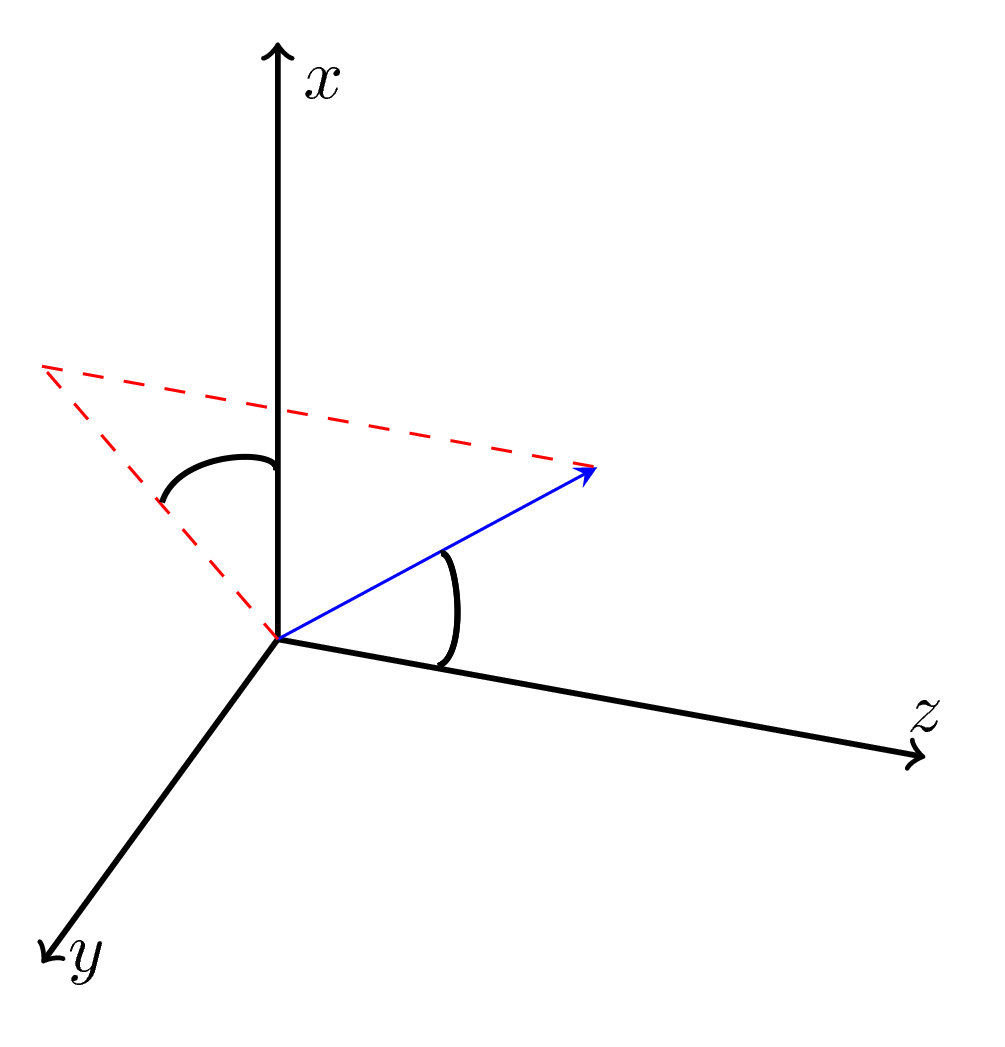
\includegraphics[width=0.2\textheight]{Figures/Geometries/coordinates.png}};
  %   \begin{scope}[x={(image.south east)},y={(image.north west)}]
  %     \node[left, text=black] at (0.27, 0.6){$\phi$};
  %     \node[right, text=black] at (0.45, 0.45){$\theta$};
  %   \end{scope}
  % \end{tikzpicture}
  \tdplotsetmaincoords{60}{120}
  \begin{tikzpicture}
    [scale=3,
      tdplot_main_coords,
      axis/.style={->,black,thick},
      vector/.style={-stealth,ForestGreen,very thick},
      vector guide/.style={dashed,ForestGreen,thick},
      angle/.style={ForestGreen,thick}]
    
    % standard tikz coordinate definition using x, y, z coords
    \coordinate (O) at (0,0,0);
    
    % tikz-3dplot coordinate definition using r, theta, phi coords
    \tdplotsetcoord{P}{.8}{55}{60}
    
    % draw axes
    \draw[axis] (0,0,0) -- (1,0,0) node[anchor=north east]{};
    \draw[axis] (0,0,0) -- (0,1,0) node[anchor=north west]{};
    \draw[axis] (0,0,0) -- (0,0,1) node[anchor=south]{};
    
    % draw a vector from O to P
    \draw[vector] (O) -- (P);
    
    % draw guide lines to components
    \draw[vector guide] (O) -- (Pxy);
    \draw[vector guide] (Pxy) -- (P);
    
    % draw an arc illustrating the angle defining the orientation
    \tdplotdrawarc[angle]{(O)}{.35}{0}{60}{anchor=north}{}
    
    % define the rotated coordinate frame to lie in the "theta plane"
    \tdplotsetthetaplanecoords{55}
    
    \tdplotdrawarc[tdplot_rotated_coords,angle]{(O)}{.35}{0}{55}
                  {anchor=south west}{}
                  
  \end{tikzpicture}
\end{figure}
\end{document}
